\chapter{Existing Solutions}

This specific part of the thesis is focused on the analysis of existing solutions provided by particular vendors that are present on the market.
It is very beneficial to be aware of solutions for adaptive authentication as there are already some companies and institutions that are trying to solve the same problem as is touched on in this thesis.

The intention behind analyzing existing solutions is to get information from the other vendors in order not to reinvent the wheel.
In order to create an optimal solution for adaptive authentication, it is advantageous to recognize common patterns in these solutions, aggregate the best parts, enhance them, and tailor them to the needs of Keycloak. 

In the following sections, there are some brief descriptions of products provided by the mentioned vendors.
The list of existing solutions and their ordering is not sorted by any particular keys but rather gathered as the most promising and exciting solutions.

\newpage
\section{Okta}

Okta is an identity management company that provides cloud-based solutions for businesses to connect people and technology securely.
Okta offers a platform that enables organizations to manage and secure user authentication, access control, and identity governance across various applications and devices.
The company's services include single sign-on, multi-factor authentication, lifecycle management, and API access management.
Okta describes its adaptive and risk-based capabilities as follows:

``User and risk levels are always changing; your security should be able to keep up.
Okta Adaptive MFA allows for dynamic policy changes and step-up authentication in response to changes in user and device behavior, location, or other contexts.''\cite{existing-okta}
\newline
\newline
Adaptive MFA supports detection and authentication challenges for riskier situations like:

\begin{itemize}
    \item Use of weak/breached passwords.
    \item Proxy use.
    \item Geographic location and zone changes.
    \item Brute force and denial-of-service attacks.
    \item Use of new/untrusted devices.
    \item Indications of anomalous behavior. 
\end{itemize}

\newpage
\subsection{Takeaways}
Okta approach introduces the consideration of external risk contexts, enhancing organizations' understanding of authentication processes by utilizing the ThreatInsight service.
This service collects information about the origin of sign-in activity directed at Okta endpoints.

ThreatInsight evaluates authentication requests by analyzing data to identify potentially suspicious activity by using machine learning and provides reasonable threat detection. 

This service furnishes critical details encompassing users, devices, locations, and networks, thereby facilitating more informed decision-making regarding access permissions.

ThreatInsight provides a way to add risk factors from external sources like third-party services. However, relying on remote services may introduce challenges, such as potential latency issues, which could impede the authentication process and lead to user frustration and operational inefficiencies.\cite{existing-okta-lowrisk} \cite{existing-okta-confidence}

Ensuring the safety and trustworthiness of these outside sources is very important.
I think leveraging the risk factors from external sources must be carefully considered in order to avoid the risk of data leaks or mistakes that could harm the authentication system.

\newpage
\section{Citrix}

Citrix Systems, Inc. is an American multinational cloud computing and virtualization technology company that provides server, application, and desktop virtualization, networking, software as a service (SaaS), and cloud computing technologies.
Citrix products were claimed to be used by over 400,000 clients worldwide, including 99\% of the Fortune 100 and 98\% of the Fortune 500.

\subsection{Takeaways}
I appreciate how Citrix Systems, Inc. adaptive authentication solution handles various details of user authentication.
It carefully considers factors such as user roles, organizational affiliations, and unique user attributes.
These factors are crucial in assessing the level of risk in each authentication attempt.
The solution does not treat each factor in isolation.\cite{existing-citrix-wiki} \cite{existing-citrix-blog}

Instead, it integrates all these details to determine the overall security of an authentication attempt.
This enhances overall security and improves the user experience by making the authentication process smoother by considering the whole context of risk factors. 

\newpage
\section{OneLogin}

OneLogin, Inc. is a cloud-based identity and access management (IAM) provider that develops a unified access management (UAM) platform for enterprise-level businesses and organizations. \cite{existing-onelogin}

\subsection{Takeaways}
I like how OneLogin, Inc. describes risk-based authentication with the leverage of machine learning. 
Such solutions learn from user behavior over time to create a detailed profile of each login habits of the user.
That includes tracking devices, typical login times, and usual work locations.
Additional analysis of IP addresses, network reputations, and threat data is used to enhance security further.

Solution SmartFactor, provided by OneLogin, Inc., gathers risk factor values described above, which are used as inputs for their Vigilance AI solution.
After analyzing these factors via the artificial intelligence engine, the contextual risk score is evaluated.
The risk score is in the range 0-100.
Based on the evaluated score, appropriate actions are executed, such as requiring additional authentication steps or denying access.\cite{existing-onelogin} 

\newpage
\section{Silverfort}
Silverfort, Inc. provides several security-related products, such as the Advanced MFA, Identity Threat Detection and Response solution, Risk-based authentication, and others.
Silverfort, Inc. was founded in 2016 by Hed Kovetz, Yaron Kassner, and Matan Fattal.
It is headquartered in Tel Aviv and has offices in the US and Singapore, as well as local Sales teams in over 18 countries across EMEA, NA, and APAC.\cite{example_silverfort}

\subsection{Takeaways}

Silverfort, Inc. provides risk-based authentication with the possibility of specifying adaptive policies.
I like the concept of adaptive policies, as it is possible to create custom authentication policies to meet unique requirements for the authentication process.

These policies can leverage risk scoring provided by the Silverfort, Inc. solution and trigger proactive security controls, such as requiring additional authentication steps or denying access. 
This concept is very flexible and provides the possibility to explicitly set particular risk indicators in order to react to specific attacks that your environment is likely to experience.

You can see an example of configuring the described adaptive policy in figure \ref{fig:silverfort-auth-policy} below.
This adaptive policy is basically a rule for the authentication process, and when conditions of the adaptive policy are met, a particular action is executed.\cite{example_silverfort}

\begin{figure}[htbp]
  \centering
  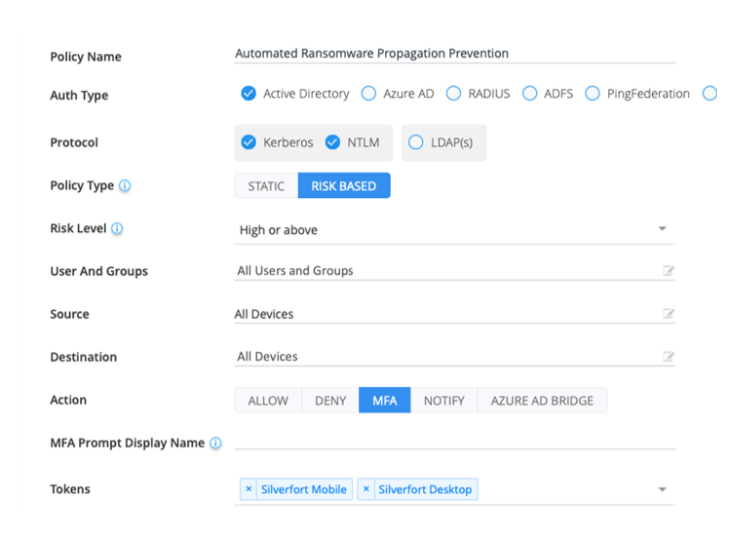
\includegraphics[width=1\textwidth]{img/silverfort-auth-policy.png}
  \caption[Silverfort Adaptive Policy]{Silverfort Adaptive Policy. Source: \cite{example_silverfort}}
  \label{fig:silverfort-auth-policy}
\end{figure}

\newpage
\section{Beyond Identity}

Beyond Identity, Inc. is a company that specializes in passwordless identity management and authentication solutions. They offer a platform that aims to eliminate the need for passwords and provide more secure and user-friendly authentication methods.

\subsection{Takeaways}
I like the concept called the triad of risk that Beyond Identity, Inc. provided in relation to adaptive (risk-based) authentication.
The triad of risk is a methodology for conceptualizing risk factors when permitting or denying access to applications.
The triad consists of three factors: \textit{Device risk}, \textit{Application risk}, and \textit{Contextual risk}.

\textit{Device Risk} involves assessing the security of the user hardware, considering factors like passcodes, authentication methods, operating system updates, the presence of firewalls, etc.
This assessment helps determine the likelihood of the device being compromised.

\textit{Application Risk} focuses on the potential impact an application access could have on operations if exploited by a malicious actor rather than the inherent riskiness of the application itself.
It considers the sensitivity of the data or functions accessible through the application.

\textit{Contextual Risk} takes into account the user behavior and environment, especially in the context of remote work.
Factors such as geographic location, typical access patterns, and time of access are considered to identify abnormal behavior that may indicate fraud or malicious intent.

Adaptive authentication uses contextual factors to evaluate access attempts, triggering alarms for deviations from established patterns.
Certain anomalies, like accessing an application from an unusual location, are given higher risk weighting.

Beyond Identity, Inc. also provides the feature of authentication and device policies.
As was stated previously, authentication policies may provide the possibility to create custom authentication policies to meet unique requirements for the authentication process.
Other than that, additional device policies provide an additional security layer as devices, that are trying to access the application, need to meet the requirements specified by these policies.

You can notice, that the user experience around configuring these policies varies as the user interface might have different representations as shown in figure \ref{fig:beyond-identity-auth-policy}. \cite{existing-beyond-identity}

\begin{figure}[htbp]
  \centering
  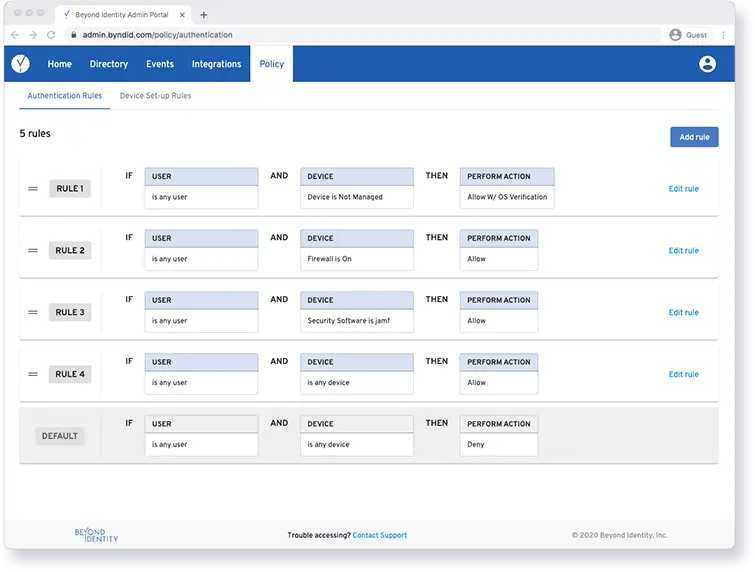
\includegraphics[width=1\textwidth]{img/beyond-auth-policy.png}
  \caption[Beyond Identity Authentication Policies]{Beyond Identity Authentication Policies. Source: \cite{existing-beyond-identity}}
  \label{fig:beyond-identity-auth-policy}
\end{figure}

\newpage